\documentclass[a4paper,14pt]{extarticle}

\usepackage[a4paper,top=20mm,bottom=20mm,left=30mm,right=10mm]{geometry}
\usepackage[T1,T2A]{fontenc}
\usepackage[utf8]{inputenc}
\usepackage[russian]{babel}
\usepackage{indentfirst}
\usepackage{titlesec}
\usepackage{graphicx}
\usepackage{verbatim}
\usepackage{fancyvrb}

\renewcommand{\baselinestretch}{1.3}

\titleformat{\section}{\normalsize\bfseries}{\thesection}{1em}{}
\titleformat{\subsection}{\normalsize\bfseries}{\thesubsection}{1em}{}

\setlength{\parindent}{12.5mm}

\begin{document}

\newpage\thispagestyle{empty}
\begin{center}
  \MakeUppercase{
    Министерство науки и высшего образования Российской Федерации\\
    Федеральное государственное бюджетное образовательное учреждение высшего образования\\
    <<Вятский Государственный Университет>>\\
  }
  Институт математики и информационных систем\\
  Факультет автоматики и вычислительной техники\\
  Кафедра электронных вычислительных машин
\end{center}
\vfill

\begin{center}
  Отчет по лабораторной работе №2\\
  по дисциплине\\
  <<Объектно-ориентированное программирование>>\\
\end{center}
\vfill

\noindent
\begin{tabular}{ll}
  Выполнил студент гр. ИВТб-2301-05-00 \hspace{5mm} & \rule[-1mm]{25mm}{0.10mm}\,/Макаров С.А./ \\
  Руководитель преподаватель                        & \rule[-1mm]{25mm}{0.10mm}\,/Шмакова Н.А./ \\
\end{tabular}

\vfill
\begin{center}
  Киров 2026
\end{center}

\newpage
\section*{\hspace{12.5mm}Цель работы}
Цель работы: изучить и освоить принципы объектно-ориентированного программирования, включая инкапсуляцию, наследование и полиморфизм, путем создания иерархии классов в выбранной предметной области, взаимодействие с базой данных и графическим интерфейсом.

\section*{\hspace{12.5mm}Задание}
На основании согласованной в первой лабораторной работе предметной области разработать приложение с  графическим интерфейсом пользователя, используя классы и особенности C\#. Сведения  об объектах предметной области необходимо хранить в БД.
\section*{\hspace{12.5mm}Решение}
Предметная область описывает управление ассортиментом блюд в заведении общественного питания. Система позволяет хранить информацию о различных блюдах, учитывать их специфические характеристики, рассчитывать итоговую цену для клиента в зависимости от этих характеристик и выводить информацию о блюде в удобном виде.

Программа содержит классы <<Dish>>, представлющий базовый класс блюда,  <<Pizza>>, наследованный от <<Dish>> и представлющий класс пиццы, <<Salad>> наследованный от <<Dish>> и представлющий класс салата.

Базовый класс <<Dish>> содержит:
\begin{itemize}
  \item[--] Свойста:
  \begin{itemize}
    \item[--] public Guid Id \{ get; \} -- свойство, означающее уникальный идентификатор;
    \item[--] public string Name \{ get; set; \} -- свойство, означающее название блюда, строковый тип данных;
    \item[--] public int Weight \{ get; set; \} -- свойство, означающее вес блюда, целочисленный тип данных;
    \item[--] public double Price \{ get; set; \} -- свойство, цена блюда, формат с плавающей запятой;
  \end{itemize}
  \item[--] Конструкторы:
  \begin{itemize}
    \item[--] public Dish(string name, int weight = 100, double price = 10.0) - публичный конструктор, принимает  в качестве параметров название, вес и цену блюда;
    \item[--] public Dish(string name) : this(name, 200, 20.0) - публичный конструктор, принимает название блюда в качестве параметра;
    \item[--] public Dish() : this("Dish") -- публичный конструктор, задает значения полей по умолчанию;
  \end{itemize}
  \item[--] Абстрактные методы:
  \begin{itemize}
    \item[--] public abstract string DisplayInfo() -- публичный абстрактный метод, возвращающий информацию о блюде, не принимает параметров;
    \item[--] public abstract double CalcFullPrice() -- публичный абстрактный метод, возвращающий полную цену блюда.
  \end{itemize}
\end{itemize}

Класс <<Pizza>>, наследованный от класса <<Dish>> содержит:
\begin{itemize}
  \item[--] Собственные свойства:
  \begin{itemize}
    \item[--] public Dough Dough \{ get; set; \} = Dough.Thick -- свойство, означающее типа теста, по умолчанию Thick;
  \end{itemize}
  \item[--] Конструкторы:
  \begin{itemize}
    \item[--] public Pizza() : base() -- публичный конструктор, задает значения полей по умолчанию;
    \item[--] public Pizza(string name) : base(name) -- публичный конструктор, принимает название пиццы в качестве параметра;
    \item[--] public Pizza(string name, int weight, double price) : base(name, weight, price) -- публичный конструктор, принимает в качестве параметров название, вес и цену пиццы;
  \end{itemize}
  \item[--] Переопределенные методы:
  \begin{itemize}
    \item[--] public override string DisplayInfo() -- публичный метод, возвращающий информацию о пицце (название, тип теста, вес, цена), не принимает параметров, возвращает информацию в следующем виде:
      \begin{Verbatim}[tabsize=4]
        Pizza: Margarita, thick dough, 450g, $18.00;
      \end{Verbatim}
    \item[--] public override double CalcFullPrice() -- публичный метод, возвращает полную цену в зависимости от типа теста (Thick: price * 1.5, Thin: price * 1.3), не принимает параметров;
  \end{itemize}
  \item[--] Собственные методы:
  \begin{itemize}
    \item[--] public void ChangeDough() -- публичный метод, меняет тип теста, не принимает параметров;
    \item[--] public void CutInSlices() -- публичный метод, нарезает пиццу на куски, не принимает параметров, возвращает информацию в следующем виде:
    \begin{Verbatim}[tabsize=4]
      Cutting the pizza into slices...;
    \end{Verbatim}
  \end{itemize}
\end{itemize}

Класс <<Salad>>, наследованный от класса <<Dish>> содержит:
\begin{itemize}
  \item[--] Собственные свойства:
  \begin{itemize}
    \item[--] public Dressing Dressing \{ get; set; \} = Dressing.OliveOil -- свойство, означающее тип заправки, по умолчанию OliveOil;
  \end{itemize}
  \item[--] Конструкторы:
  \begin{itemize}
    \item[--] public Salad() : base() -- публичный конструктор, задает значения полей по умолчанию;
    \item[--] public Salad(string name) : base(name) -- публичный конструктор, принимает название салата в качестве параметра;
    \item[--] public Salad(string name, int weight, double price) : base(name, weight, price) -- публичный конструктор, принимает в качестве параметров название, вес и цену салата;
  \end{itemize}
  \item[--] Переопределенные методы:
  \begin{itemize}
    \item[--] public string DisplayInfo() override -- публичный метод, отображает информацию о салате (название, тип заправки, вес, цена), не принимает параметров, возвращает информацию в следующем виде:
    \begin{Verbatim}[tabsize=4]
Salad: Caesar, OliveOil dressing, 250g, $12.60;
    \end{Verbatim}
    \item[--] public double CalcFullPrice() override -- публичный метод, возвращает полную цену в зависимости от типа заправки (OliveOil: price * 1.4, Mayonnaise: price * 1.3), не принимает параметров;
  \end{itemize}
  \item[--] Собственные методы:
  \begin{itemize}
    \item[--] public void ChangeDressing() -- публичный метод, меняет тип заправки, не принимает параметров;
    \item[--] public string TossWithDressing() -- публичный метод, перемешивает салат с заправкой, не принимает параметров, возвращает информацию в следующем виде:
    \begin{Verbatim}[tabsize=4]
Tossing the salad with OliveOil...;
    \end{Verbatim}
  \end{itemize}
\end{itemize}

Диаграмма классов сущностей представлена на рисунке 1.

\pagebreak
\begin{figure}[ht]
  \centering
  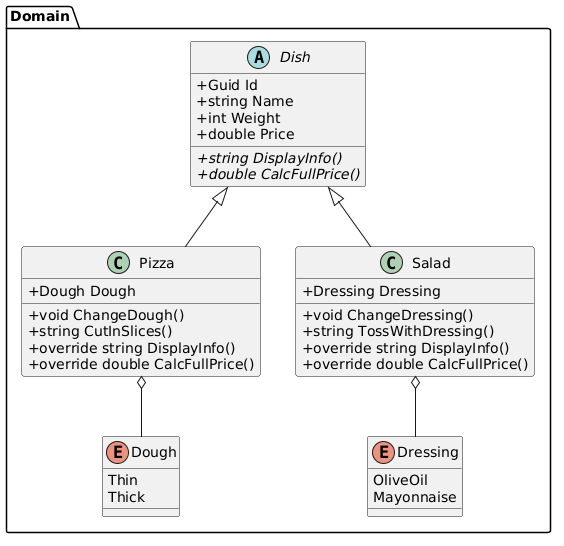
\includegraphics[width=1\linewidth]{img/uml-1.png}
\end{figure}
\begin{center}
  Рисунок 1 – Диаграмма классов сущностей
\end{center}

Разработаны серверные и клиентское приложение в виде веб-интерфейса. Серверное приложение содержит подключение к базе данных, конфигурацию моделей и контроллеры.

Подключение к базе даныых Postgres происходит с помощью следующей строки подключения:
\begin{Verbatim}[tabsize=4]
"ConnectionStrings": {
  "LabaratoryDbContext": "User ID=root;Password=root;
            Host=localhost;Port=5432;Database=labaratory_cs;"
}
\end{Verbatim}

Далее регистрируется контекст общения с базой данных в главном файле:
\begin{Verbatim}[tabsize=4]
builder.Services.AddDbContext<LabaratoryDbContext>(options =>
{
    options.UseNpgsql(builder.Configuration.GetConnectionString(nameof(LabaratoryDbContext)));
});
\end{Verbatim}

И сам класс контекста:
\begin{Verbatim}[tabsize=4]
public class LabaratoryDbContext(
    DbContextOptions<LabaratoryDbContext> options) : DbContext(options)
{
    public DbSet<Pizza> Pizzas { get; set; }
    public DbSet<Salad> Salads { get; set; }

    protected override void OnModelCreating(ModelBuilder modelBuilder)
    {
        modelBuilder.ApplyConfiguration(new PizzaConfiguration());
        modelBuilder.ApplyConfiguration(new SaladConfiguration());

        base.OnModelCreating(modelBuilder);
    }
}
\end{Verbatim}

Конфигурация сущности, например для <<Pizza>> содержит метод Configure(), в котором описываются поля сущности для базы данных:
\begin{Verbatim}[tabsize=4]
public class PizzaConfiguration : IEntityTypeConfiguration<Pizza>
{
    public void Configure(EntityTypeBuilder<Pizza> builder)
    {
        builder.HasKey(p => p.Id);

        builder.Property(p => p.Name);
        builder.Property(p => p.Weight);
        builder.Property(p => p.Price);

        builder.Property(p => p.Dough)
               .HasConversion(
                    d => d.ToString(),
                    d => Enum.Parse<Dough>(d)
               );
    }
}
\end{Verbatim}

Следующим шагом идёт создание контроллера для ответов на запросы для клиентов. Класс <<PizzasController>> наследуется от класса <<Controller>>.

Содержит следующие методы:
\begin{itemize}
  \item[--] public async Task<IActionResult> CreateAsync([FromBody] CreatePizzaRequest request) -- метод, который создает новую запись о пицце;
  \item[--] public async Task<IActionResult> GetAllAsync() -- метод, возвращающий весь список пицц, хранящаеся в базе данных;
  \item[--] public async Task<IActionResult> GetByIdAsync([FromRoute] Guid id) -- метод, возвращающий отдельную запись о пицце по уникальному идентификатору;
  \item[--] public async Task<IActionResult> CutAsync([FromRoute] Guid id) -- метод, возвращающий сообщение о нарезании пиццы на кусочки по уникальному идентификатору;
  \item[--] public async Task<IActionResult> DisplayInfoAsync([FromRoute] Guid id) -- метод, возвращающий полное описание записи пиццы по уникальному идентификатору;
  \item[--] public async Task<IActionResult> GetFullPriceAsync([FromRoute] Guid id) -- метод, возвращающий полную стоимость пиццы по уникальному идентификатору;
  \item[--] public async Task<IActionResult> UpdateAsync([FromRoute] Guid id, [FromBody] UpdatePizzaRequest request) -- метод, который обновляет записи о пицце по уникальному идентификатору;
  \item[--] public async Task<IActionResult> ChangeDressingAsync([FromRoute] Guid id) -- метод, меняющий тип теста пиццы по уникальному идентификатору;
  \item[--] public async Task<IActionResult> DeleteAsync([FromRoute] Guid id) -- метод, удаляющий запись о пицце по уникальному идентификатору.
\end{itemize}

Конфигурация и контроллер для сущности <<Salad>> выполняется аналогичным способом и содержат аналогичные методы.

Диаграмма классов контроллеров и конфигураций сущностей представлены на рисунке 2.

\begin{figure}[ht]
  \centering
  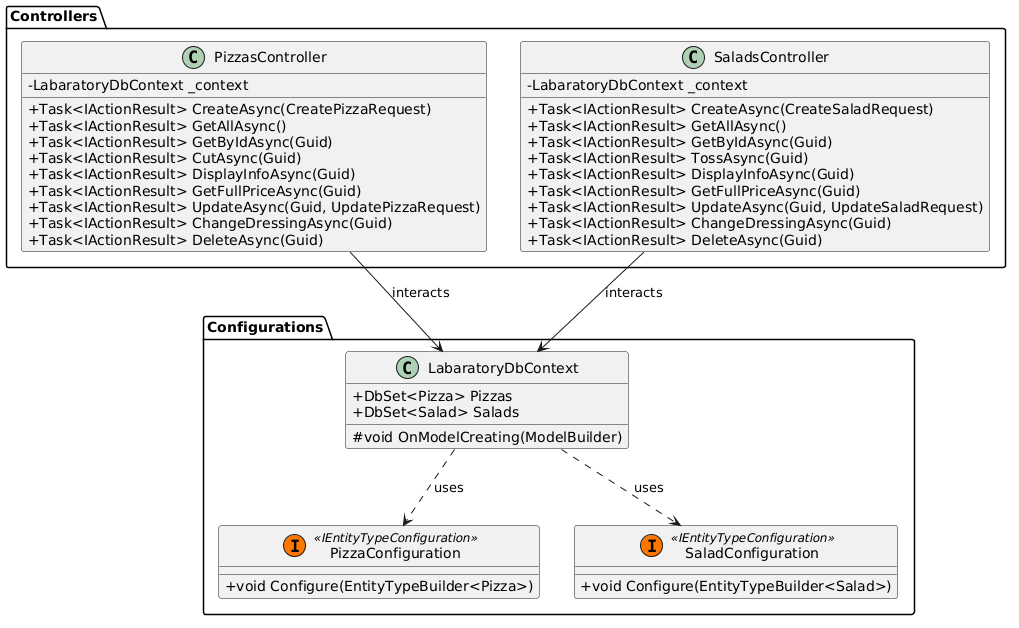
\includegraphics[width=1\linewidth]{img/uml-2.png}
\end{figure}
\begin{center}
  Рисунок 1 – Диаграмма классов контроллеров и конфигураций
\end{center}

Также разработан веб-интерфейс для взаимодействия с WEB API, экранные формы которого представлены на рисунках 3, 4.

\pagebreak
\begin{figure}[ht]
  \centering
  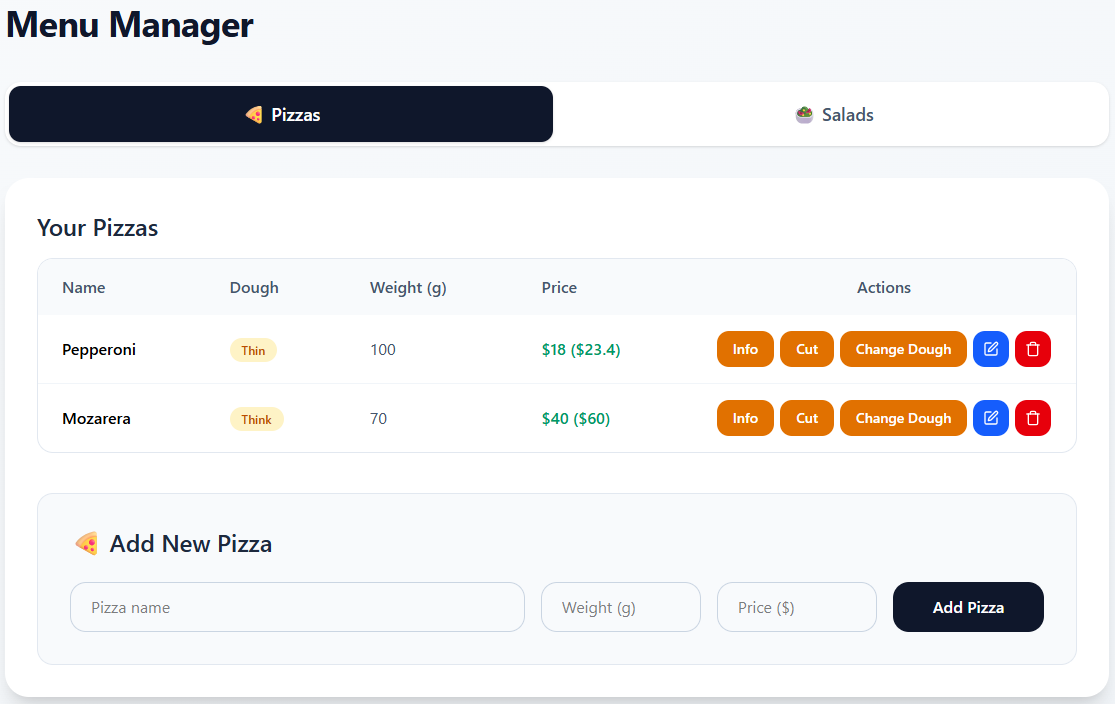
\includegraphics[width=0.88\linewidth]{img/form-1.png}
\end{figure}
\begin{center}
  Рисунок 3 – Экранная форма отображения и создания записей
\end{center}

\begin{figure}[ht]
  \centering
  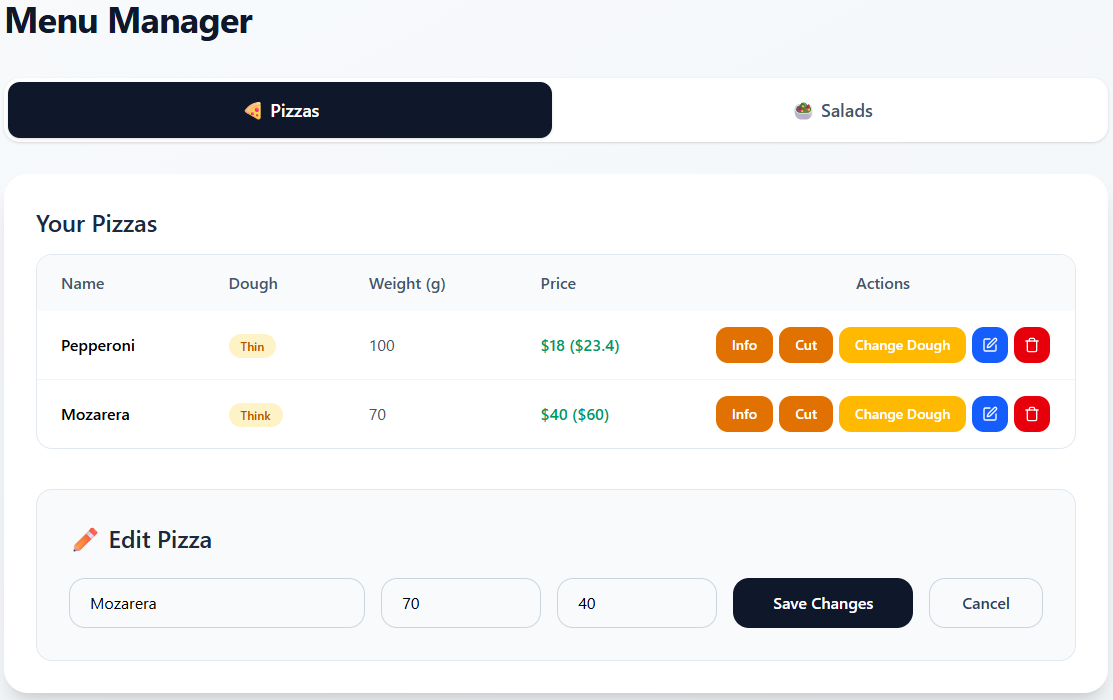
\includegraphics[width=0.88\linewidth]{img/form-2.png}
\end{figure}
\begin{center}
  Рисунок 4 – Экранная форма редактирования записей
\end{center}

\section*{\hspace{12.5mm}Вывод}
В ходе выполнения лабораторной работы была разработана и реализована иерархия классов, моделирующая управление ассортиментом блюд в заведении общественного питания. Изучены основные принципы объектно-ориентированного программированя: инкапсуляция, наследование, полиморфизм. Разработана база данных и веб-приложение, демонстрирующее применение данных принципов.

\end{document}